\section[Využití výzkumných reaktorů]{Využití výzkumných reaktorů jako zdrojů neutronů}

Výzkumné jaderné reaktory hrají klíčovou roli v rozvoji jaderné vědy a technologií. Na rozdíl od energetických reaktorů, jejichž primární účel je výroba elektřiny, výzkumné reaktory slouží především k experimentálním, vzdělávacím a vývojovým účelům. Jsou navrženy tak, aby umožnily detailní studium neutronových polí, testování nových konstrukčních materiálů, vývoj jaderného paliva a získávání cenných dat pro validaci výpočetních metod a simulací.

Tyto reaktory také poskytují neutronové zdroje pro aplikace v medicíně (např. produkce radionuklidů pro diagnostiku a terapii), průmyslu (neutronová radiografie) a vědě (materiálový výzkum pomocí neutronového rozptylu). Díky své flexibilitě a schopnosti simulovat různé provozní podmínky hrají nezastupitelnou roli při řešení aktuálních výzev spojených s jadernou bezpečností, udržitelností a inovacemi v oblasti jaderné energetiky.

V České republice se výzkumné reaktory staly významnou součástí jaderného výzkumu. Mezi nejvýznamnější zařízení patří reaktory LVR-15, LR-0 v Řeži a VR-1, VR-2, které poskytují zázemí pro experimentální měření, přípravu odborníků a mezinárodní spolupráci. Výzkumné reaktory tak nejen podporují technický pokrok, ale také přispívají k mezinárodnímu sdílení poznatků a k budoucímu rozvoji celého oboru.

Informace ohledně způsobů využití jednotlivých výzkumných reaktorů na světě lze dohledat v databázi IAEA, Research Reactor Database. Nachází se tam veškeré informace ohledně vše výzkumných reaktorů, ve vše provozních stavech (plánované, ve výstavbě, v provozu, krátkodobě odstavené, dlouhodobě odstavené I vyřazené z provozu). 

Způsoby využití lze rozdělit například podle toho, jestli se využívá přímo AZ reaktoru (uvnitř reaktoru) nebo jestli je reaktor pouze jako zdroj neutron (vně reaktoru). Tak trochu mimo leží vzdělávání a výcvik:

\begin{table}[h!]
\centering
\caption{Výzkumné reaktory v provozu, dočasně odstavené, plánované a ve výstavbě.}
\begin{tabular}{lrr}
\toprule
Stav reaktoru & Počet reaktorů & Počet zemí \\
\midrule
Celkem & 257 & 56 \\
Výuka / školení & 161 & 51 \\
Neutronová aktivační analýza & 116 & 50 \\
Výroba radioizotopů & 82 & 41 \\
Materiální ozařování & 68 & 26 \\
Neutronová radiografie & 69 & 37 \\
Neutronový rozptyl & 44 & 28 \\
Dopování křemíku & 23 & 15 \\
Geochronologie & 24 & 21 \\
Barvení drahokamů & 20 & 12 \\
Zachytávání neutronů borem pro terapii & 15 & 12 \\
Inovativní výzkum energie &  &  \\
Příprava jaderných dat & 16 & 9 \\
Další aplikace & 116 & 34 \\
\bottomrule
\end{tabular}
\end{table}

\subsection{Neutronová aktivační analýza}

Neutronová aktivační analýza (NAA) je jaderná analytická technika využívaná pro stanovení:

\begin{itemize}
    \item Složení vzorků
    \item Nečistot ve vzorcích
    \item Stopových prvků ve vzorcích
\end{itemize}

NAA umožňuje získat jak kvalitativní, tak kvantitativní výsledky. Stabilní nuklidy po interakci s neutrony mohou vytvářet nestabilní izotopy. Tyto nestabilní izotopy jsou následně analyzovány pomocí vícekanálového analyzátoru. 

Z detekované gama záření lze určit původní stabilní nuklidy, které byly ve vzorku přítomny před jeho ozářením. Tato technika je velmi užitečná pro přesné analýzy složení vzorků a sledování příměsí či stopových prvků.

Existuje několik typů neutronové aktivační analýzy, z nichž každá má specifické aplikace a vlastnosti:

\begin{itemize}
    \item \textbf{Instrumentální NAA (INAA)}: Standardní metoda bez chemické separace.
    \item \textbf{Cyklická instrumentální NAA (CINAA)}: Používá opakované cykly ozařování a měření.
    \item \textbf{Epithermální instrumentální NAA (EINAA)}: Využívá epithermální neutrony.
    \item \textbf{Radiochemická NAA (RNAA)}: Zahrnuje chemickou separaci před měřením.
    \item \textbf{Předkoncentrační NAA (PNAA)}: Před analýzou je prováděna předkoncentrace vzorku.
    \item \textbf{Odvozená NAA (DNAA)}: Modifikace zahrnující derivace vzorku.
    \item \textbf{Promptní gama NAA (PGNAA)}: Detekce gama záření během ozařování.
    \item \textbf{Zpožděná gama NAA (DGNAA)}: Detekce gama záření po určitém zpoždění od ozařování.
\end{itemize}

NAA má širokou škálu využití např. v archeologii, geologii, geochemii, biomedicíně, nutriční a zdravotní vědě, a vědách týkající se životního prostředí. Příklady z VR-1: tibetské mince, zdravotní doplňky, mamutí kosti enviromentální vzorky, vzorky lidské tkáně atd.

\subsection{Ozařování materiálů}

Ozařování materiálů se provádí z různých oblastech např. testování nových typů paliv, změny materiálu vlive záření, teploty, tlaku atd. především pro použití v jaderných elektrárnách nebo nových typech reaktorů.

Lze použít speciální ozařovací místa, speciální smyčky s prostředím, tlakové nádoby atd.

\subsection{Měření jaderných dat}

Výzkumné reaktory mohou být také používány k ověřování jaderných dat -- data ze štěpení (výtěžky ze štěpení), data účinných průřezů, data o zpožděných neutronech, rozpadová data atd.

\subsection{Produkce radioizotopů}

Radioizotopy jsou používány v široké škále aplikací -- medicína, průmysl, zemědělství, věda a výzkum. Příklady nejpoužívanějších radioizotopů jsou:
\textsuperscript{14}C, \textsuperscript{24}Na, \textsuperscript{32}P, \textsuperscript{35}S, \textsuperscript{38}Cl, \textsuperscript{41}Ar, \textsuperscript{51}Cr, \textsuperscript{56}Mn, \textsuperscript{60}Co, \textsuperscript{54}Cu, \textsuperscript{89}Sr, \textsuperscript{99m}Tc, \textsuperscript{125}I, \textsuperscript{131}I, \textsuperscript{133}Xe, \textsuperscript{153}Sm, \textsuperscript{169}Yb, \textsuperscript{170}Tm, \textsuperscript{192}Ir, \textsuperscript{198}Au, \textsuperscript{177}Lu.

Pro nemedicínské aplikace jsou nejčastěji produkovány dva radioizotopy: \textsuperscript{60}Co a \textsuperscript{192}Ir (zdroje gama záření). Tyto izotopy jsou používány v oblastech jako gama zobrazování, gama radioterapie, kalibrační zařízení, sterilizace nástrojů apod. 

V medicínské oblasti je nejčastěji používán \textsuperscript{99m}Tc z \textsuperscript{99}Mo. Tento izotop se využívá v 80\,\% případů diagnostiky nádorů pomocí radioizotopů. \textsuperscript{99}Mo vzniká jako produkt ze štěpení \textsuperscript{235}U. Uranový vzorek je ozářen v reaktoru, kde vznikne štěpením \textsuperscript{99}Mo, který je následně přepracován do tekuté formy.

    \[
        {}^{99}_{42}\mathrm{Mo} \xrightarrow{\beta^-} {}^{99m}_{43}\mathrm{Tc} \xrightarrow{\gamma} {}^{99}_{43}\mathrm{Tc}
    \]
    \[
        T_{1/2} = 66.924\,\mathrm{h}, \quad T_{1/2} = 6.0072\,\mathrm{h}
    \]

\begin{figure}[H]
    \centering
    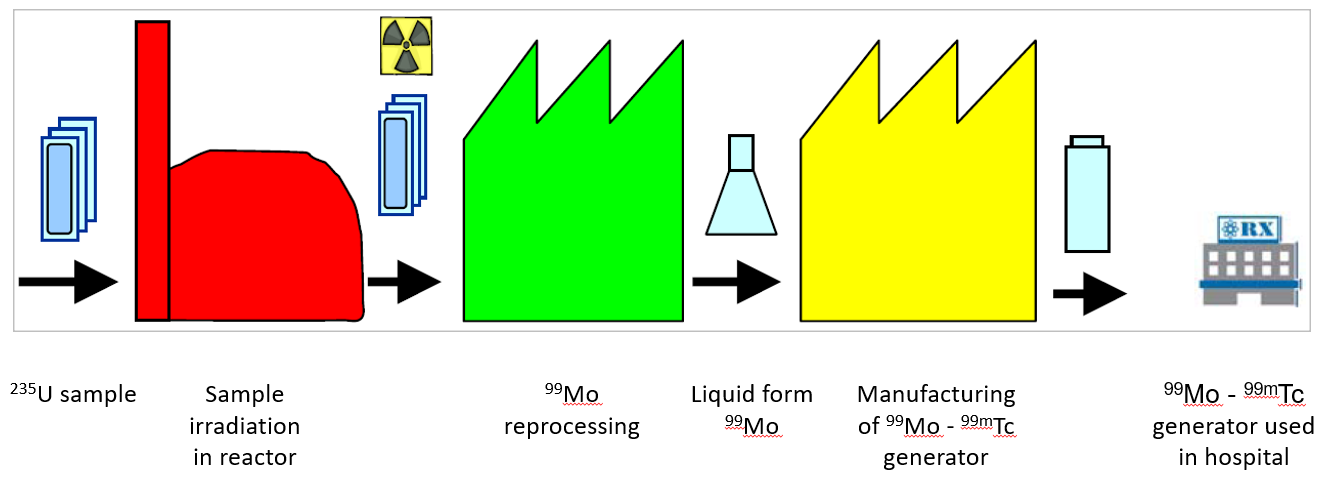
\includegraphics[width=0.7\linewidth]{img/CestaRadioizotopu.png}
    \caption{Cesta radioizotopu}
    \label{fig:enter-label}
\end{figure}

Jsou potřebné vysoké neutronové toky, přibližně $10^{13} - 10^{14}\,\mathrm{n/s/cm^2}$. V současnosti provozované reaktory pro produkci \textsuperscript{99}Mo jsou: BR2 (Belgie), HRF (Nizozemsko), LVR-15 (Česko), OPAL (Austrálie), MARIA (Polsko), RA-3 (Argentina), Itálie (Pavia)

\subsection{Transmutace -- dopování křemíku a barvení kamenů}

\textbf{Dopování křemíku:}

Během ozařování křemíkových ingotů tepelnými neutrony v reaktoru dochází ke vzniku nečistot, což zlepšuje vodivost křemíkového polovodiče. Přírodní křemík obsahuje cca 3 \% $^{30}$Si, který je vhodný k dopování. 

 \[
{}^{30}_{14}\mathrm{Si} + {}^{1}_{0}\mathrm{n} \rightarrow {}^{31}_{14}\mathrm{Si} + \gamma
\quad \text{a} \quad
{}^{31}_{14}\mathrm{Si} \rightarrow {}^{31}_{15}\mathrm{P} + \beta^-
\]

Křemík je čtyřmocný prvek, zatímco fosfor je pětimocný. Když se v matrici krystalů křemíku vytvoří fosfor, čtyři z jeho valenčních elektronů vytvoří vazby podobné okolním atomům křemíku a extra valenční elektron se uvolní. Tento volný elektron v krystalu je dostupný jako volný nosič náboje, který mění vodivost krystalu.

Křemík je k tomuto nejvhodnější, ale existují i jiné materiály např. germanium. Opět jsou potřeba vysoké neutronového toky cca 10$^{13}$ - 10$^{14}$ n/s.cm$^2$. 

\textbf{Barvení drahých kamenů:}

Barvení drahokamů je založeno na myšlence, že po ozáření mohou některé drahokamy změnit svou barvu na atraktivnější a hodnotnější. 

Ozáření může být provedeno rychlými neutrony nebo vysokoenergetickým gama zářením. Nádoby jsou stíněné (bór, kadmium) za účelem potlačení ozáření tepelnými neutrony a použití pouze rychlých neutronů (10$^{13}$ - 10$^{14}$ n/s.cm$^2$). Po ozáření je nutné nechat klesnou aktivitu, doba zaleží na typu kamenů, ale obvykle několik měsíců.

Drahé kameny se obvykle vkládají do ozařovacího kontejneru o hmotnosti asi 2 kg kamenů, které se nakládají k aktivní zóně. Dominantně je ozařován topaz, který po ozáření mění barvu z bílé/průhledné na modrou. V některých zemích je barvení drahokamů zakázáno. V Řeži to dělali, ale už to mají zakázané.

\subsection{Neutronové zobrazování}

Neutronové zobrazování je metoda určená k pozorování vnitřních struktur neprůhledných objektů. Jedná se o nedestruktivní metodu. Funguje na stejném principu jako rentgenové zobrazování. Rozdíl je pouze v interakci neutronu s látkou, což poskytuje jiný kontrast než rentgen. Mezi další zobrazovací metody patří například:

\begin{itemize}
    \item Rentgenové zobrazování
    \item Gama zobrazování
\end{itemize}

\begin{figure}[H]
    \centering
    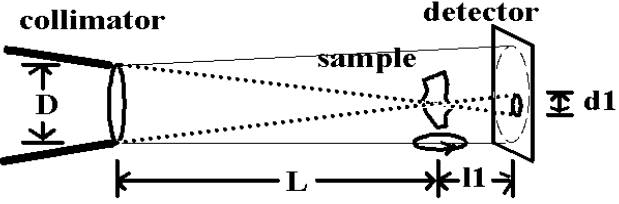
\includegraphics[width=0.7\linewidth]{img/SestavanaNZ.png}
    \caption{Neutronové zobrazování}
    \label{fig:enter-label}
\end{figure}

Základní princip: Intenzita paprsku je po průchodu zobrazovaným objektem utlumena v závislosti na tloušťce a materiálu objektu. Útlum je dán materiálovým složením vzorku -- míra pravděpodobnosti interakce je dána účinným průřezem. Toto zeslabení závisí na:

\begin{itemize}
    \item Tloušťce objektu
    \item Materiálu, ze kterého je objekt vyroben
\end{itemize}

Existuje několik metod NI (neutron imaging): neutronová radiografie (2D zobrazování -- vytváří se pouze 2D obraz zobrazovaného předmětu), neutronová počítačová tomografie (3D zobrazování -- pomocí sady 2D obrazů pod různými úhly lze počítačově provést 3D rekonstrukci obrazu), stroboskopické zobrazování (zobrazování dynamických procesů). Nově patří do neutronového zobrazování i další pokročilé metody: energeticky selektivní zobrazování (používá se velmi úzké neutronové spektrum), neutronová mřížková interferometrie, zobrazování pomocí polarizovaných neutronů, zobrazování ve vysokém rozlišení.

Dříve se používaly jako detektory fotografické filmy s konvertorem neutronů, v současnosti se používají digitální systémy založení na kombinaci kamera (CCD nebo CMOS) scintilátor. 

NI má širokou škálu použití např. archeologie, kulturní dědictví, jaderný průmysl, výzkum palivových článků, výzkum baterií, environmentální věda -- rostliny, průmyslové výrobky atd.

\begin{figure}[H]
    \centering
    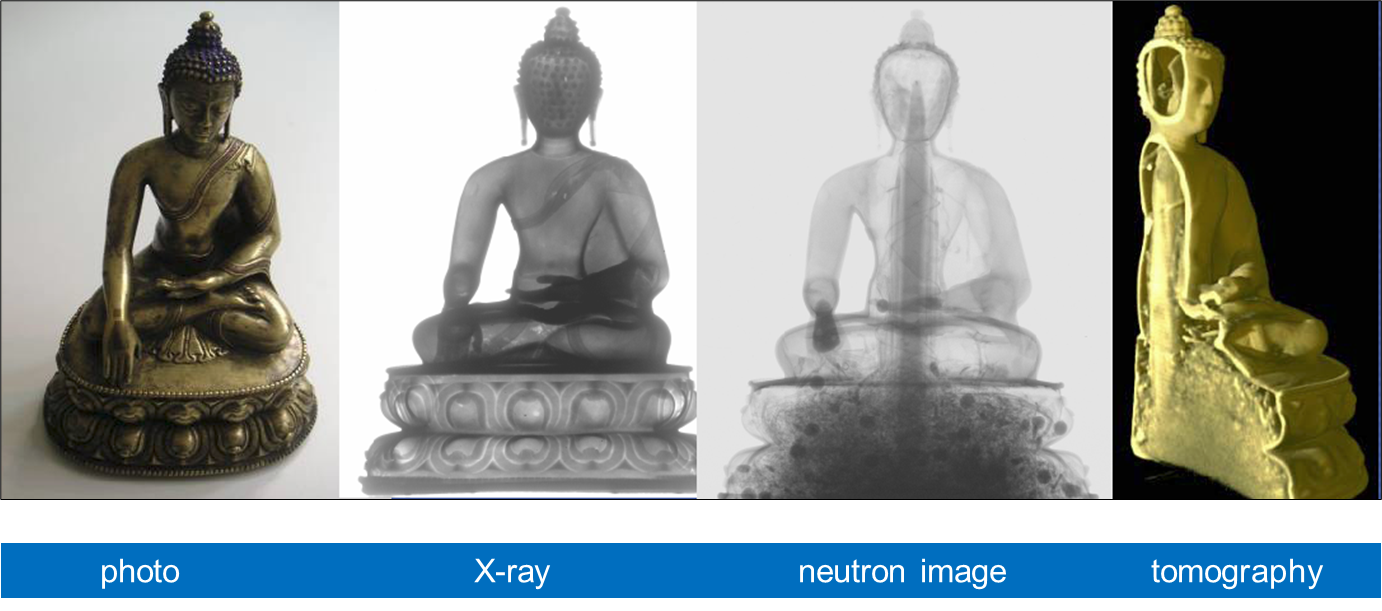
\includegraphics[width=0.7\linewidth]{img/Zobrazování.png}
    \caption{Příklady prosvícení neutrony.}
    \label{fig:Zobra}
\end{figure}

\begin{figure}
    \centering
    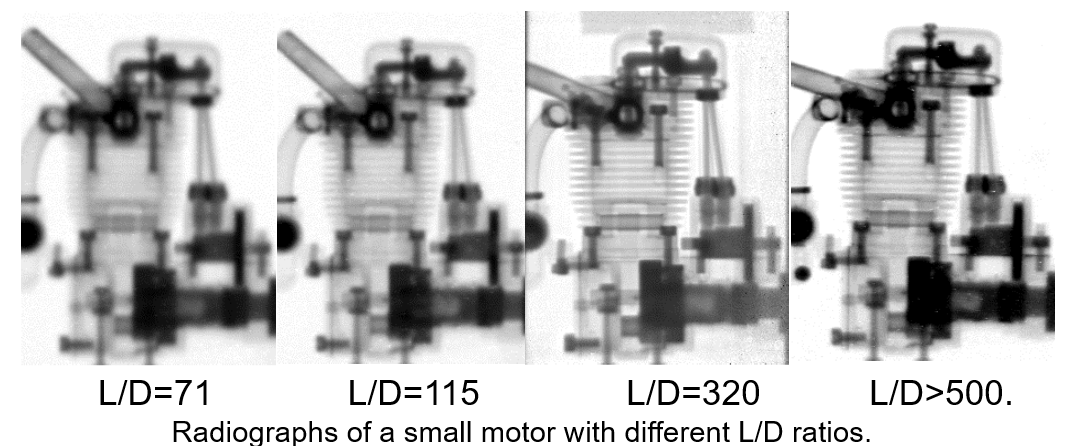
\includegraphics[width=0.5\linewidth]{img/RozlišeníPodleLD.png}
    \caption{Rozlišení podle L/D}
    \label{fig:enter-label}
\end{figure}

\subsection{Rozptylové reakce}

Rozptylové aplikace jsou založeny na částicově-vlnové dualitě neutronů. Zkoumání materiálu je založeno především na koherentním rozptylu neutronů. Tepelné neutrony mají vlnovou délku podobnou meziatomovým vzdálenostem, díky tomuto jevu je možné určovat vzdálenosti mezi jednotlivými atomy. Neutrony nemají náboj, proto se dostanou snáze do vnitřních struktur materiálů. 

Příkladem rozptylových aplikací je neutronová difrakce -- jedná se o pružný koherentní rozptyl, který se řídí Braggovým zákonem. Dalším příklady jsou rozptyl do malých úhlů (SANS -- small angle neutron scattering) a zpětný rozptyl (back scattering). 

\begin{figure}[H]
    \centering
    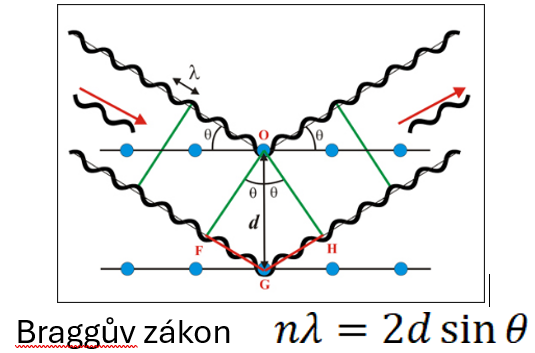
\includegraphics[width=0.5\linewidth]{img/Braggův zákon.png}
    \caption{Braggův zákon.}
    \label{fig:enter-label}
\end{figure}

Rozptylové aplikace se používají především v oblasti materiálového výzkumu, jako jsou fyzika a chemie kondenzovaných látek, nanotechnologie, věda o polymerech, výzkum udržitelné energie, senzory a chytré materiály atd.

Svazky můžou být vyvedeny i mimo hlavní budovu rekatoru. 

\begin{figure}[H]
    \centering
    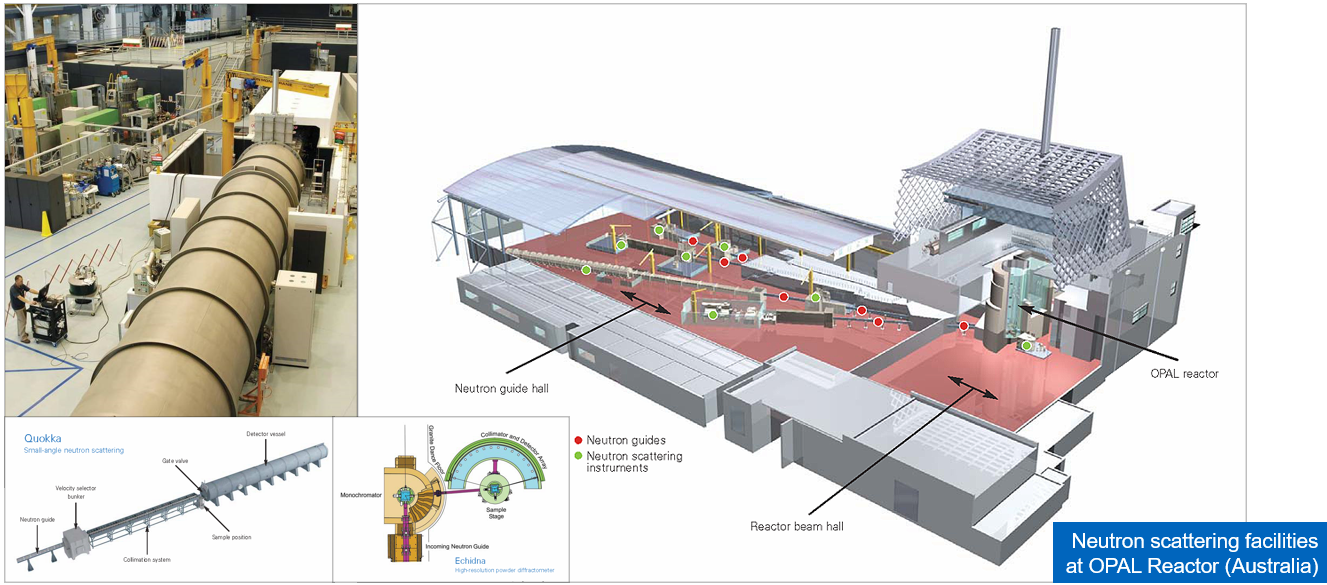
\includegraphics[width=0.75\linewidth]{img/OPALScattering.png}
    \caption{OPAL Scattering}
    \label{fig:enter-label}
\end{figure}

\subsection{Borová záchytová terapie}

Borová záchytová terapie je určena především k léčbě nádorů hlavy a krku. Je založena na interakci neutronového svazku s $^{10}$B, který je umístěn do speciálního roztoku. Ten je absorbován nádorem, který je poté bombardován svazkem neutronů. Dochází k (n, $\alpha$) reakci a vzniklé alpha záření poškozuje okolní nádorovou tkáň. 

Klinické studie byly provedeny v řadě zemí: Japonsko, Spojené státy americké, Finsko, Švédsko, Česká republika, Argentina. Současný trend je přesouvat léčbu z výzkumných reaktorů na urychlovače, které mohou být umístěny přímo v nemocnicích a poskytnou příjemnější prostředí pro pacienty. 

\subsection{Vzdělávání a školení}

Výzkumné reaktory poskytují vynikající možnosti pro vzdělávání i školení. Jsou vhodné pro výuku studentů na všech úrovních univerzitního vzdělávání a pro školení odborníků z průmyslu a výzkumných institucí. Mezi klíčové skupiny, které mohou těžit z výcviku na výzkumných reaktorech, patří:

\begin{itemize}
    \item Personál jaderných elektráren
    \item Personál výzkumných reaktorů
    \item Inspektoři regulačních orgánů
    \item Inspektoři radiační ochrany z různých organizací
    \item Hasičské záchranné sbory
\end{itemize}

Výzkumné reaktory jsou obzvláště vhodné pro jaderné vzdělávání studentů na všech třech úrovních akademického vzdělání. Výzkumné reaktory podporují široké spektrum studijních programů.

Výzkumné reaktory slouží také jako cenný nástroj pro zapojení veřejnosti, umožňují exkurze a návštěvy, které podporují porozumění jaderné vědě a technologii.